\documentclass{beamer}

\usepackage[export]{adjustbox}
\usepackage{amsmath,amsthm,amssymb,amsfonts}
\usepackage[backend=biber, style=apa]{biblatex}
\usepackage[T1]{fontenc}
\usepackage{graphicx}
\usepackage{lmodern}
\usepackage[outputdir=dist]{minted}
\usepackage{ru}
\usepackage{url}
\usepackage{xpatch,letltxmacro}
\usepackage{stmaryrd}

\newcommand{\cd}[1]{\texttt{#1}}

\setminted{fontsize=\small}
\LetLtxMacro{\cminted}{\minted}
\let\endcminted\endminted
\xpretocmd{\cminted}{\RecustomVerbatimEnvironment{Verbatim}{BVerbatim}{}}{}{}

\mode<presentation>{}

\title{\textbf{Compiler Construction: Lexical analyses}}

\author{Quinten Cabo, Marijn van Wezel}

\institute{Radboud University Nijmegen}
\date{27 February 2024}

\begin{document}

\frame{\titlepage}

\begin{frame}
  \frametitle{What was a compiler again?}
  
  \begin{center}
  \only<1>{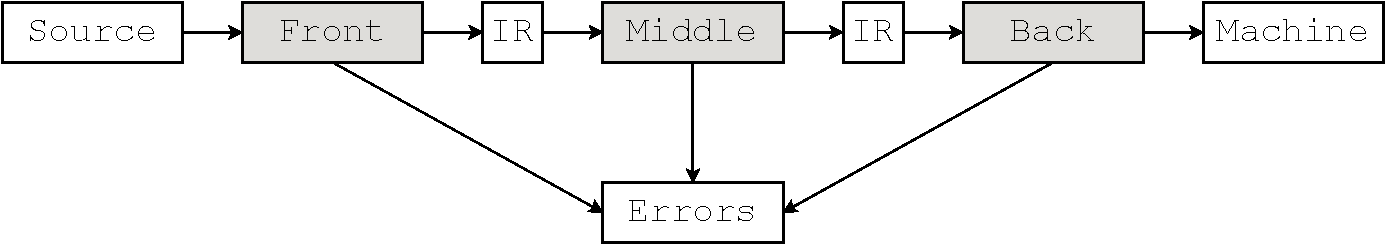
\includegraphics[width=300px]{figures/compiler_phases.pdf}}
  \only<2>{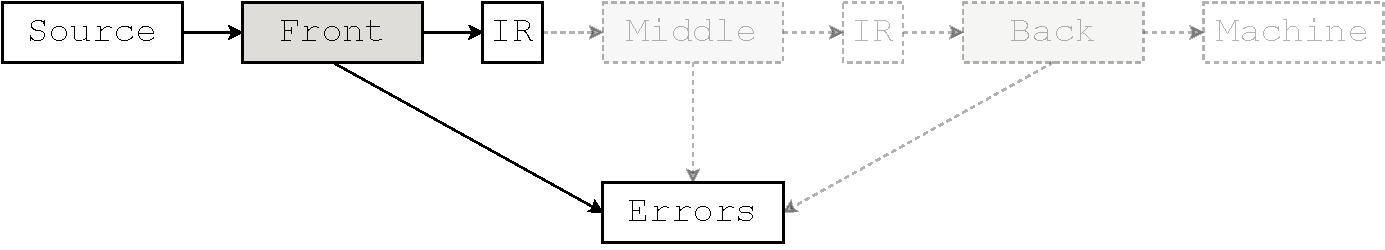
\includegraphics[width=300px]{figures/compiler_phases_highlighted.pdf}}
  \end{center}
\end{frame}

\begin{frame}
  \begin{center}Questions?\end{center}
\end{frame}

\end{document}

